\documentclass{article}
\usepackage{graphicx}
\usepackage{amsmath}   
\usepackage{amsthm}
\usepackage{tikz}
\usepackage{pgfplots}
\pgfplotsset{compat=1.18}
\setlength{\parindent}{0pt}

\title{90-S1-Q9 \\ Solution + Discussion}
\author{David Puerta}
\date{}

\begin{document}

\maketitle

\begin{abstract}
    \noindent In this document we will go through the solution to the 90-S1-Q9 question and provide a discussion of the question at the end. There are also hints on the first page to aid you in finding a solution. There is no single method that results in an answer to a STEP question, there are a multitude of different paths that end up at the same solution. However, some methods are more straight forward and you are encouraged to take the path of least resistance.  
\end{abstract}

\vspace{1cm}

\begin{center}
    \textbf{Hints}
\end{center}

\textbf{First part}: Find the equation of the tangents at $A$ and $B$ then form simultaneous equations. 

\vspace{1cm}

\textbf{Second part}:  Draw a sketch of the trapeziums.

\vspace{1cm}

\textbf{Third part}: Consider the area of both trapeziums, the area under the curve and the rectangle formed of unit height.



\newpage

\begin{center}
    \textbf{Solution}
\end{center}

\vspace{0.5cm}

Differentiating the curve $y=\frac{1}{x}$,
\[
\frac{\mathrm{d}y}{\mathrm{d}x} = -\frac{1}{x^2}
\]
to get the gradients of the tangents at $A:m_a=-1$ and $B:m_b=-1/b^2$. Finding the equations of the tangents,
\begin{align*}
& \text{Tangent at $A$: } y = -x+2 \\
& \text{Tangent at $B$: } y = -\frac{1}{b^2}x+\frac{2}{b} 
\end{align*}
and solving 
\[
 -x+2 = -\frac{1}{b^2}x+\frac{2}{b}
\]
to find the $x$-coordinate of $C$ as $x=\frac{2b}{b+1}$. This gives the coordinates of $C$,
\[
C:\left(\frac{2b}{b+1},\frac{2}{b+1}\right).
\]

\vspace{0.5cm}

Drawing a diagram of the points and the curve,
\begin{figure}[h!]
\centering
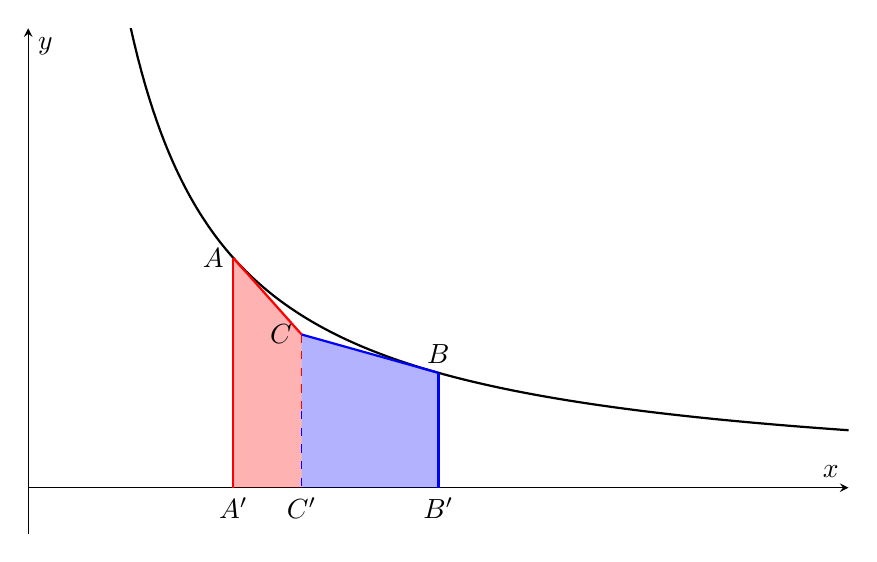
\begin{tikzpicture}[scale=1]
    \begin{axis}[
        axis lines=middle,
        xmin=0, xmax=4,
        ymin=-0.2, ymax=2,
        samples=200,
        xlabel={$x$},
        ylabel={$y$},
        domain=0.25:4,
        ticks=none,
        width=12cm,
        height=8cm
    ]
        \addplot[black, thick] {1/x};

        \fill[red, opacity=0.3] 
            (axis cs:1,1) -- 
            (axis cs:1,0) -- 
            (axis cs:1.333333,0) -- 
            (axis cs:1.333333,0.666666) -- 
            cycle;

        \fill[blue, opacity=0.3] 
            (axis cs:1.333333,0.6666666) -- 
            (axis cs:1.333333,0) -- 
            (axis cs:2,0) -- 
            (axis cs:2,0.5) -- 
            cycle;

        \node[left] at (axis cs:1,1) {$A$};
        \node[right,above] at (axis cs:2,0.5) {$B$};
        \node[left] at (axis cs:1.333333,0.6666666) {$C$};

        \draw[thick,red] (axis cs:1,1) -- (axis cs:1.333333,0.666666);
        \draw[thick,red] (axis cs:1,1) -- (axis cs:1,0);
                
        \draw[dashed,red] (axis cs:1.333333,0.666666) -- (axis cs:1.333333,0.333333);
        \draw[dashed,blue] (axis cs:1.333333,0.333333) -- (axis cs:1.333333,0);

        \draw[thick,blue] (axis cs:1.333333,0.666666) -- (axis cs:2,0.5);
        \draw[thick,blue] (axis cs:2,0.5) -- (axis cs:2,0);

        \node[below] at (axis cs:1,0) {$A'$};
        \node[below] at (axis cs:1.333333,0) {$C'$};
        \node[below] at (axis cs:2,0) {$B'$};
    \end{axis}
\end{tikzpicture}
\end{figure}

shows the two quadrilaterals we are after. Finding the area of $ACC'A'$,
\[
\text{Area of $ACC'A'$} =  \frac{1}{2} \times (CC' + AA') \times (C'-A')
\]
where $CC'$ and $AA'$ are the side lengths and $C'-A'$ is the bottom length of the quadrilateral. Simplifying,
\begin{align*}
& \text{Area of $ACC'A'$} =  \frac{1}{2} \times \left(\frac{2}{b+1} + 1\right) \times \left(\frac{2b}{b+1} - 1\right) \\
& = \frac{(b+3)(b-1)}{2(b+1)^2}.
\end{align*}
Similarly, finding the area of $CBB'C'$,
\[
\text{Area of $CBB'C'$} =  \frac{1}{2} \times (BB' + CC') \times (B'-C')
\]
where $BB'$ and $CC'$ are the side lengths and $B'-C'$ is the bottom length of the quadrilateral. Simplifying,
\begin{align*}
& \text{Area of $CBB'C'$} =  \frac{1}{2} \times \left(\frac{1}{b} + \frac{2}{b+1}\right) \times \left(b-\frac{2b}{b+1}\right) \\
& = \frac{(3b+1)(b-1)}{2(b+1)^2}.
\end{align*} 

\vspace{0.5cm}

Notice that for $b>1$, the following figure
\begin{figure}[h!]
\centering
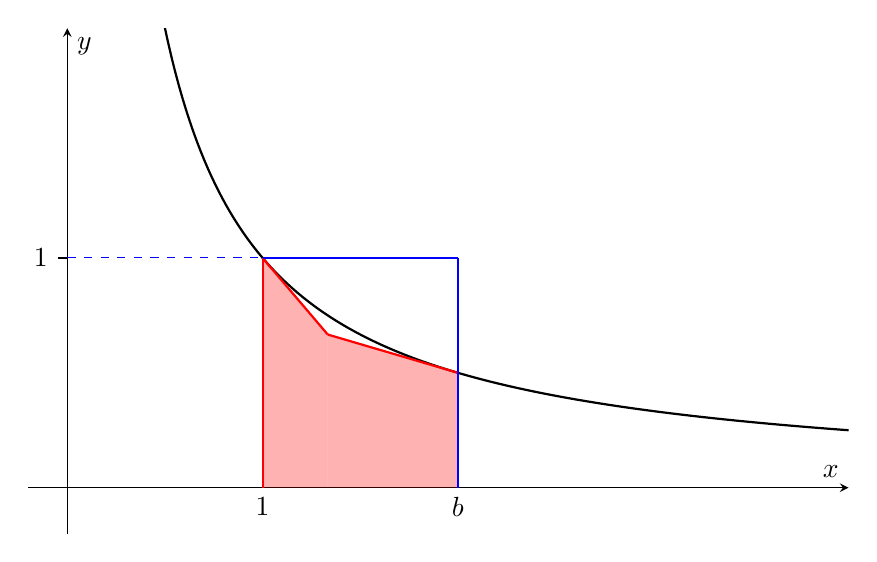
\begin{tikzpicture}[scale=1]
    \begin{axis}[
        axis lines=middle,
        xmin=-0.2, xmax=4,
        ymin=-0.2, ymax=2,
        samples=200,
        xlabel={$x$},
        ylabel={$y$},
        domain=0.25:4,
        ticks=none,
        width=12cm,
        height=8cm
    ]
        \addplot[black, thick] {1/x};

        \fill[red, opacity=0.3] 
            (axis cs:1,1) -- 
            (axis cs:1,0) -- 
            (axis cs:1.333333,0) -- 
            (axis cs:1.333333,0.666666) -- 
            cycle;

        \fill[red, opacity=0.3] 
            (axis cs:1.333333,0.6666666) -- 
            (axis cs:1.333333,0) -- 
            (axis cs:2,0) -- 
            (axis cs:2,0.5) -- 
            cycle;

        \draw[thick,red] (axis cs:1,1) -- (axis cs:1.333333,0.666666);
        \draw[thick,red] (axis cs:1,1) -- (axis cs:1,0);

        \draw[thick,red] (axis cs:1.333333,0.666666) -- (axis cs:2,0.5);
        \draw[thick,red] (axis cs:2,0.5) -- (axis cs:2,0);

        \draw[thick,blue] (2,0) -- (2,1);
        \draw[thick,blue] (1,1) -- (2,1);

        \node[below] at (2,0) {$b$};
        \node[below] at (1,0) {$1$};
        \node[left] at (-0.05,1) {$1$};

        \draw[thick] (-0.05,1) -- (0,1);

        \draw[dashed,blue] (0,1) -- (1,1);
    \end{axis}
\end{tikzpicture}
\end{figure}

shows three areas: the red shape, the area under the graph $y=\frac{1}{x}$ between $x=1$ and $x=b$ and the blue rectangle. Finding the area of the red shape,
\[
\text{Area of the red shape } = \frac{(b+3)(b-1)}{2(b+1)^2} + \frac{(3b+1)(b-1)}{2(b+1)^2} = \frac{2(b-1)}{b+1}
\]
the area under the graph,
\[
\text{Area under the graph } = \int_{1}^{b} \frac{1}{x} \,\mathrm{d}x = \ln(b)
\]
and the area of the rectangle,
\[
\text{Area of the rectangle } = 1 \times (b-1) = b-1
\]
gives the inequality
\[
\frac{2(b-1)}{b+1} \leq \ln(b) \leq b-1.
\]
Letting $z = b-1$ (with $b>1 \Rightarrow z>0$),
\[
\frac{2z}{z+2} \leq \ln(z+1) \leq z
\]
for $z>0$.

\newpage

\begin{center}
    \textbf{Discussion}
\end{center}

\vspace{0.5cm}

The hardest part of this question is completing the construction of the three areas needed to obtain the final inequality. This use of the three geometric areas in a diagram, the area of some shape under the curve, the area under the curve and the area of some shape above the curve, is typical when constructing such inequalities. Most of the case you are given the hardest area to find (typically the shape underneath or above) and have to construct the other two - as in this case. It is a good idea when trying to find the third shape to try to find the simplest shape that is above the curve, such as a square,  triangle or other polygons. Once you identify the areas to consider, the rest is quite straight forward. Another instance of this three area argument to construct an inequality is in 04-S3-Q3 where a similar argument is used to find an inequality of the integral of a convex function.\par

\quad Other aspects of this question are standard to those who are comfortable with coordinate geometry. Overall, this question is a pretty standard coordinate geometry question. 


\end{document}
